\section{Motivação}

\subsection{Sistemas de Recomendação}

\abbrev{RS}{sistemas de recomendação}
Sistemas de recomendação (RS, do inglês \textit{recommender systems}) são
ferramentas de \textit{software} que sugerem itens úteis para um usuário
\cite{ricci2010introduction}. Esses sistemas, que podem ser personalizados ou
não-personalizados, ajudam usuários a lidarem com processos de tomada de decisão
em meio a sobrecarga de informações, seja na escolha de um produto em um
\textit{e-commerce} ou na seleção de um filme em um serviço de
\textit{streaming}. Ao contrário de uma ferramenta de busca em que o usuário
ativamente procura por um item específico, sistemas de recomendação são úteis
quando o usuário explora um catálogo diversificado, otimizando a
distribuição dos itens a partir de suas preferências pessoais.

\begin{figure}[ht]
    \centering
    \includegraphics[width=0.8\textwidth]{chapters/chap01/images/spotify.png}
    \caption{Recomendações de \textit{playlists} no Spotify em Agosto de 2023.}
    \label{fig:spotify}
\end{figure}


Personalização é o processo de coleta e uso de informações pessoais para
distribuir conteúdo de forma única a um usuário, atendendo suas necessidades
percebidas pelo serviço ou declaradas explicitamente pelo usuário
\cite{liang2006personalized}. Recomendações não-personalizadas distribuem o
conteúdo recomendado de forma igualitária para todos os usuários. Uma
recomendação a partir da lista de reportagens mais lidas em um portal de
notícias é um exemplo de recomendação não-personalizada
\cite{falk2019practical}.



\begin{figure}[ht]
    \centering
    \includegraphics[width=0.6\textwidth]{chapters/chap01/images/tt.png}
    \caption{Recomendações de perfis de usuário no Twitter em Agosto de 2023.}
    \label{fig:twitter}
\end{figure}

\subsection{Sobrecarga de informação}
A sobrecarga de informação, segundo \citet{roetzel2019information}, é um estado em que um tomador de decisões observa um
conjunto ou uma carga de informações de complexidades distintas, a qual inibe a
capacidade do tomador de decisões de determinar de forma ótima a melhor decisão
possível. O uso subótimo de informações é causado
pela limitação de recursos individuais escassos. Um recurso escasso pode ser uma
característica individual (como capacidade de processamento em série, memória de
curto prazo) ou equipamento relacionado à tarefa (por exemplo, orçamento ou
tempo para tomar uma decisão). A probabilidade de alcançar a melhor decisão
possível é definida como o desempenho de tomada de decisão. A correspondência
entre a carga de informação e o desempenho da tomada de decisão é ilustrada na
Figura \ref{fig:u_invertida} \cite{roetzel2019information}.


\vspace{0.2cm}
\begin{figure}[h]
    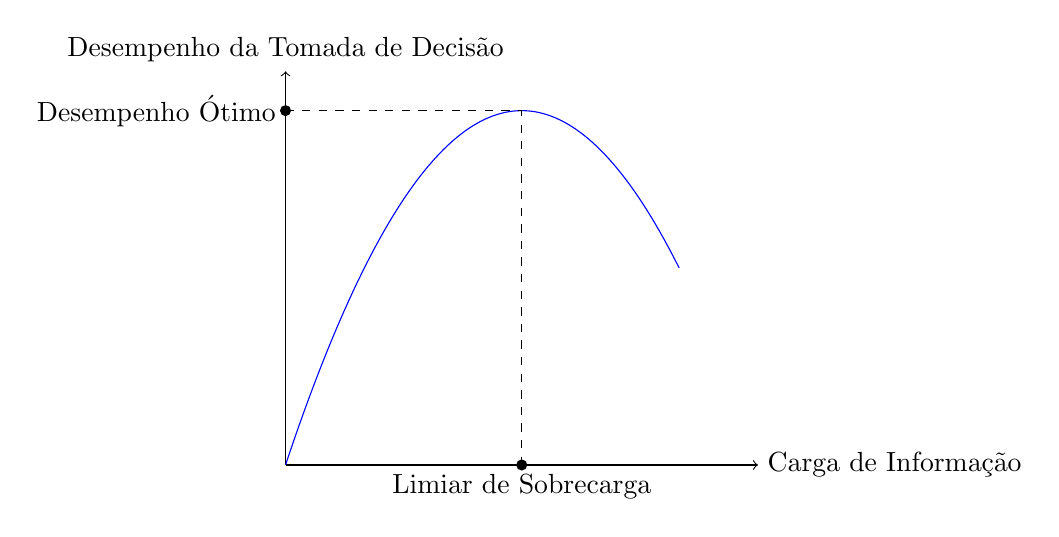
\begin{tikzpicture}
    % Eixo X
    \draw[->] (0,0) -- (6,0) node[right] {Carga de Informação};
    % Eixo Y
    \draw[->] (0,0) -- (0,5) node[above] {Desempenho da Tomada de Decisão};
  
    % Curva U invertida
    \draw[blue, domain=0:5, samples=100] plot (\x, {3*\x - 0.5*\x*\x});
  
    % Pontos de interesse
    \fill (0,4.5) circle (2pt) node[left] {Desempenho Ótimo};
    \fill (3,0) circle (2pt) node[below] {Limiar de Sobrecarga};

    % Linhas tracejadas
    \draw[dashed] (0,4.5) -- (3,4.5);
    \draw[dashed] (3,0) -- (3,4.5);
  \end{tikzpicture}
   % Descrição
    \caption{Correspondência entre a carga de informação e o desempenho da tomada
    de decisão.}
    \label{fig:u_invertida}
\end{figure}
\vspace{0.2cm}

Experimentos realizados por \citet{liang2006personalized} mostraram que, ao
avaliar a satisfação de voluntários com um sistema de recomendação de notícias,
a precisão do conteúdo recomendado sob personalização e o número de itens
recomendados influenciam diretamente na satisfação do usuário, reduzindo a
sobrecarga de informação e a insatisfação gerada pela sobrecarga.

\subsection{Indaband}

Indaband é uma aplicação móvel para distribuição e gravação de música
colaborativa e remota \cite{indaband}. A versão inicial foi disponibilizada
publicamente em Agosto de 2022. O quadro de funcionários é majoritariamente
brasileiro, enquanto que o produto possui distribuição global.

Na aplicação, usuários podem criar sessões, que são ambientes colaborativos de
gravação entre os participantes. As sessões contam com ferramentas para gravação
e mixagem. O ambiente de pré-visualização, edição e produção da sessão chama-se
\textit{Studio}.
\vspace{0.2cm}

\begin{figure}[h]
    \centering
    \subfigure[]{\includegraphics[width=0.24\textwidth]{chapters/chap01/images/inda/inda3.PNG}}
    \subfigure[]{\includegraphics[width=0.24\textwidth]{chapters/chap01/images/inda/inda.PNG}}
    \subfigure[]{\includegraphics[width=0.24\textwidth]{chapters/chap01/images/inda/inda2.PNG}}
    \subfigure[]{\includegraphics[width=0.24\textwidth]{chapters/chap01/images/inda/inda4.PNG}}
    \caption{Exemplos de telas: (a) \textit{Home} (b) \textit{Feed} (c)
    \textit{Feed} (d) \textit{Studio}.}
    \label{fig:cap_tela}
\end{figure}

Uma vez que o usuário conclua as etapas de produção da sessão no \textit{Studio}
e esteja satisfeito com o resultado final, ele tem a opção de publicar a sessão
no \textit{Feed} público da aplicação. No \textit{Feed}, todos os usuários da
plataforma podem visualizar e interagir com a sessão publicada
adicionando comentários, compartilhando com outros usuários dentro e fora da
aplicação, etc.
\vspace{0.6cm}

\subsection{Sistemas de Recomendação Baseados em Sessão}

% Sistemas de Recomendação Baseados em Sessão (SBRS, do inglês
% \textit{session-based recommender systems}) são sistemas de recomendação que 
Abordagens mais tradicionais em sistemas de recomendação modelam as interações
usuário-item na forma de uma matriz esparsa de avaliações, em que cada linha
representa um usuário e cada coluna representa um item. A tarefa em questão se
resume ao preenchimento dos valores faltantes da matriz, a depender da
abordagem escolhida \cite{}. Valores preenchidos com avaliações altas são recomendados
ao usuário, uma vez que ele ainda não os consumiu.

Por mais que a matriz de avaliações seja uma forma intuitiva de representação,
viabilizando uma boa variedade de modelos, trata-se de uma forma que
desconsidera o contexto temporal das interações ou a sequência específica de
itens que determinado usuário interagiu. Sistemas de Recomendação Baseados em
Sessão (SBRS, do inglês \textit{session-based recommender systems}) atuam
justamente nesse cenário.

Os SBRS se caracterizam por terem seus dados representados em sequências
temporalmente ordenadas de interações. Essas sequências são chamadas sessões. O
objetivo de um SBRS é prever a próxima interação do usuário durante uma sessão
em andamento.


    

\begin{figure}[h]
    \centering
    \begin{tikzpicture}
        % Define the matrix
        \matrix (m) [matrix of nodes,
                    %  nodes in empty cells,
                     column sep=-\pgflinewidth,  % Adjust cell spacing
                     row sep=-\pgflinewidth,     % Adjust cell spacing
                     nodes={draw, text width=2.5em, align=center, minimum height=2.5em, minimum width=2.5em}] {
            5 & 4 & 1 & 1 \\
            4 & 4 & 1 & 1 \\
            1 & 2 &  & 4 \\
            1 & 1 & 4 & 4 \\
        };
      
        % % Labels on the left
        \foreach \row/\label in {1/Gilberto, 2/Maria, 3/Gal, 4/Caetano} {
          \node[left] at (m-\row-1.west) {\label};
        }
      
        % % Labels on the top
        \foreach \col/\label in {1/TV, 2/DVD, 3/sal, 4/pipoca} {
          \node[above,
          ] at (m-1-\col.north) {\label};
        }
      \end{tikzpicture}
    \caption{Matriz de avaliações para produtos de um comércio eletrônico. A predição atua sobre as avaliações faltantes.}
\end{figure}

\begin{figure}[h]
    \centering
        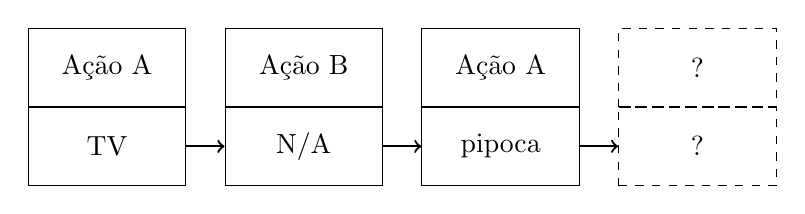
\begin{tikzpicture}
        % Draw the list cells
        \node[draw, rectangle, minimum width=2cm, minimum height=1cm] (cell1) at (0, 0) {TV};
        \node[draw, rectangle, minimum width=2cm, minimum height=1cm] (cell2) at (2.5, 0) {N/A};
        \node[draw, rectangle, minimum width=2cm, minimum height=1cm] (cell3) at (5, 0) {pipoca};
        \node[draw, dashed, rectangle, minimum width=2cm, minimum height=1cm] (cell4) at (7.5, 0) {?};

        % Draw the arrow
        \draw[->, thick] (cell1.east) -- (cell2.west);
        \draw[->, thick] (cell2.east) -- (cell3.west);
        \draw[->, thick] (cell3.east) -- (cell4.west);

        % % Add label to the left of the first cell
        % \node[left] at (cell1.west) {Sessão 1};

        % Draw the top cells with actions
        \node[draw, rectangle, minimum width=2cm, minimum height=1cm] (topcell1) at (0, 1.0) {Ação A};
        \node[draw, rectangle, minimum width=2cm, minimum height=1cm] (topcell2) at (2.5, 1.0) {Ação B};
        \node[draw, rectangle, minimum width=2cm, minimum height=1cm] (topcell3) at (5, 1.0) {Ação A};
        \node[draw, dashed, rectangle, minimum width=2cm, minimum height=1cm] (topcell4) at (7.5, 1.0) {?};

    \end{tikzpicture}
    \caption{Exemplo de uma sessão em andamento. A predição atua sobre a interação subsequente.}
\end{figure}

Cada interação das sessões está associada a tuplas que contém um ou mais dos
seguintes dados: a ação executada, o item alvo da ação, o instante em que a ação
foi executada e o usuário responsável pela ação. Por exemplo, uma sessão pode
representar uma lista ordenada de itens selecionada por um usuário anônimo, ou
uma lista de ações desempenhadas por usuários de uma mesma sessão, sem que essas
ações estejam necessariamente atreladas cada uma a um item. Isso é um aspecto
útil dos SBRS, por prover recomendações em aplicações em que não há
distinção entre usuários, ou quando as preferências de longo prazo de um
usuário novo da plataforma não foram identificadas.
\vspace{0.4cm}